
\documentclass{article}
\usepackage{tikz}

\begin{document}

\begin{center}
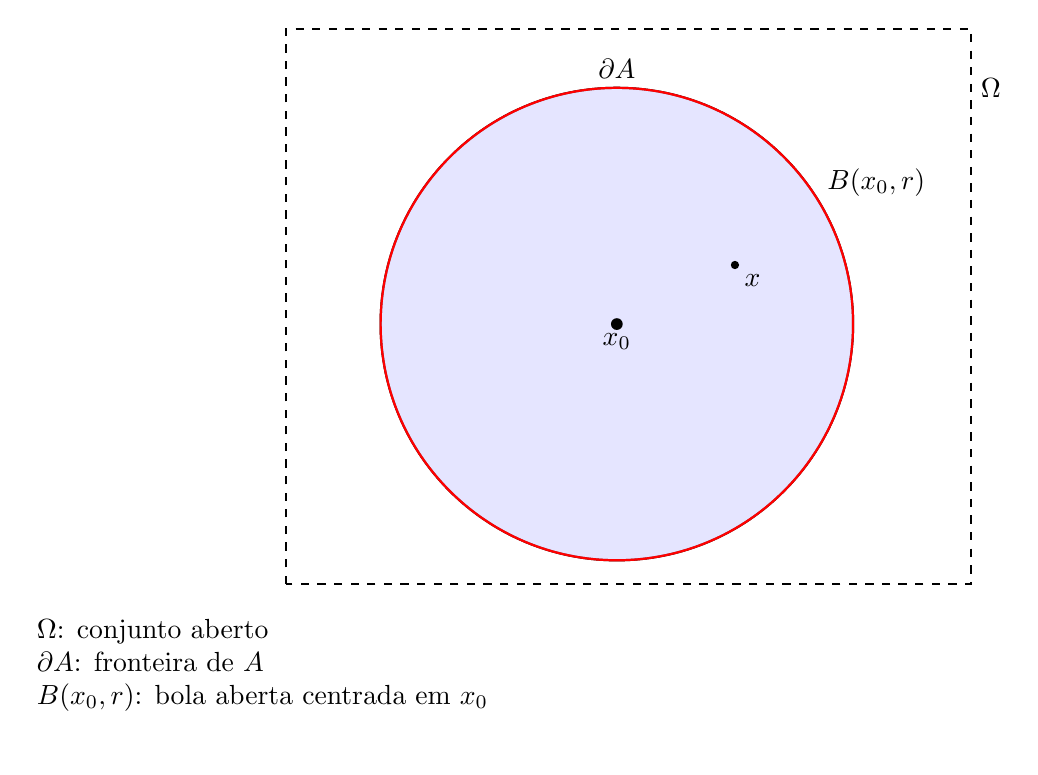
\begin{tikzpicture}[scale=1.5]

% Bola aberta B(x0, r)
\draw[thick] (0,0) circle (2cm);
\fill[blue!20,opacity=0.5] (0,0) circle (2cm);
\node at (0,0) [circle,fill=black,inner sep=1.5pt] {};
\node[below] at (0,0) {$x_0$};
\node[right] at (1.7,1.2) {$B(x_0, r)$};

% Conjunto aberto \Omega
\draw[thick,dashed] (-2.8,-2.2) rectangle (3,2.5);
\node[right] at (3,2) {$\Omega$};

% Fronteira
\draw[thick,red] (0,0) circle (2cm);
\node[above] at (0,2) {$\partial A$};

% Marcador de outro ponto no interior
\fill[black] (1,0.5) circle (1pt);
\node[below right] at (1,0.5) {$x$};

% Texto explicativo
\node at (-3,-3) [align=left] {
$\Omega$: conjunto aberto\\
$\partial A$: fronteira de $A$\\
$B(x_0, r)$: bola aberta centrada em $x_0$\\
};

\end{tikzpicture}
\end{center}

\end{document}
